\chapter{Diskussion}

\section{Anziehendes und abstoßendes Potenzial: Lokale Minima und Oszillationen}

Eine Eigenschaft der Potenzialfunktion mit anziehendem und abstoßendem Potenzial ist die Konvergenz des Gradientenabstiegsverfahren zu einem lokalen Minimum bei konkaven Hindernissen.
Davon betroffen sind Occupancy Grids, deren Hindernisse Polygone mit überstumpfen Winkeln ($180\text{°} \le \text{Winkel} \le 360\text{°}$) bilden.
Bekannte Beispiele der Literatur sind C- und U-förmige Polygone \cite{maqbool.2021, yujiang.2017}:
\begin{figure}[h!]
	\centering
	\footnotesize
	\centerline{\resizebox{0.3\linewidth}{!}{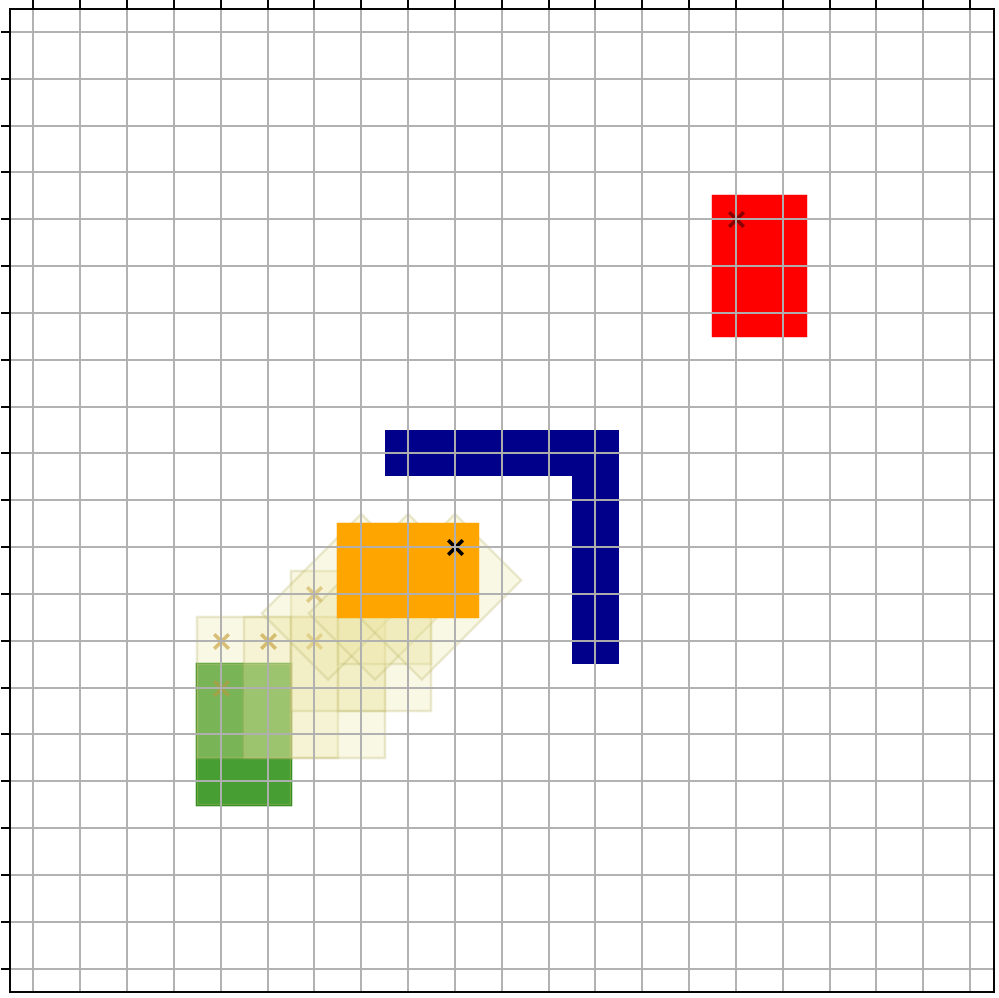
\includegraphics{bilder/attr-repul-c-shape.png}}}
	\caption{Für konkave Hindernisse konvergiert das Gradientenabstiegsverfahren mit anziehendem und abstoßendem Potenzial.}
\end{figure}

Weiterhin führt das Gravitationsfeld von Potenzialfeldern mit anziehendem und abstoßendem Potenzial zwischen Hindernisengstellen zu Oszillationen. Der Roboter wechselt bei dieser Art des lokalen Minimums zwischen zwei Koordinaten mit entgegen gerichteten Gradienten.
Insbesondere kleine Occupancy Grids sind von diesem Effekt betroffen, da die Grenzen des Potenzialfelds als Hindernisse berücksichtigt werden. Abbildung \ref{fig:oscillation} zeigt diesen Effekt Anhand des Potenzialfelds aus Kapitel X (TODO).
Die Erhöhung des Abstandes zwischen Occupancy-Grid-Grenzen und Hindernissen vermeidet dieses Problem.

\begin{figure}[h!]
	\footnotesize
	\centering
	\hspace*{\fill}
	\begin{minipage}{0.46\textwidth}%
		\centerline{\resizebox{0.6\linewidth}{!}{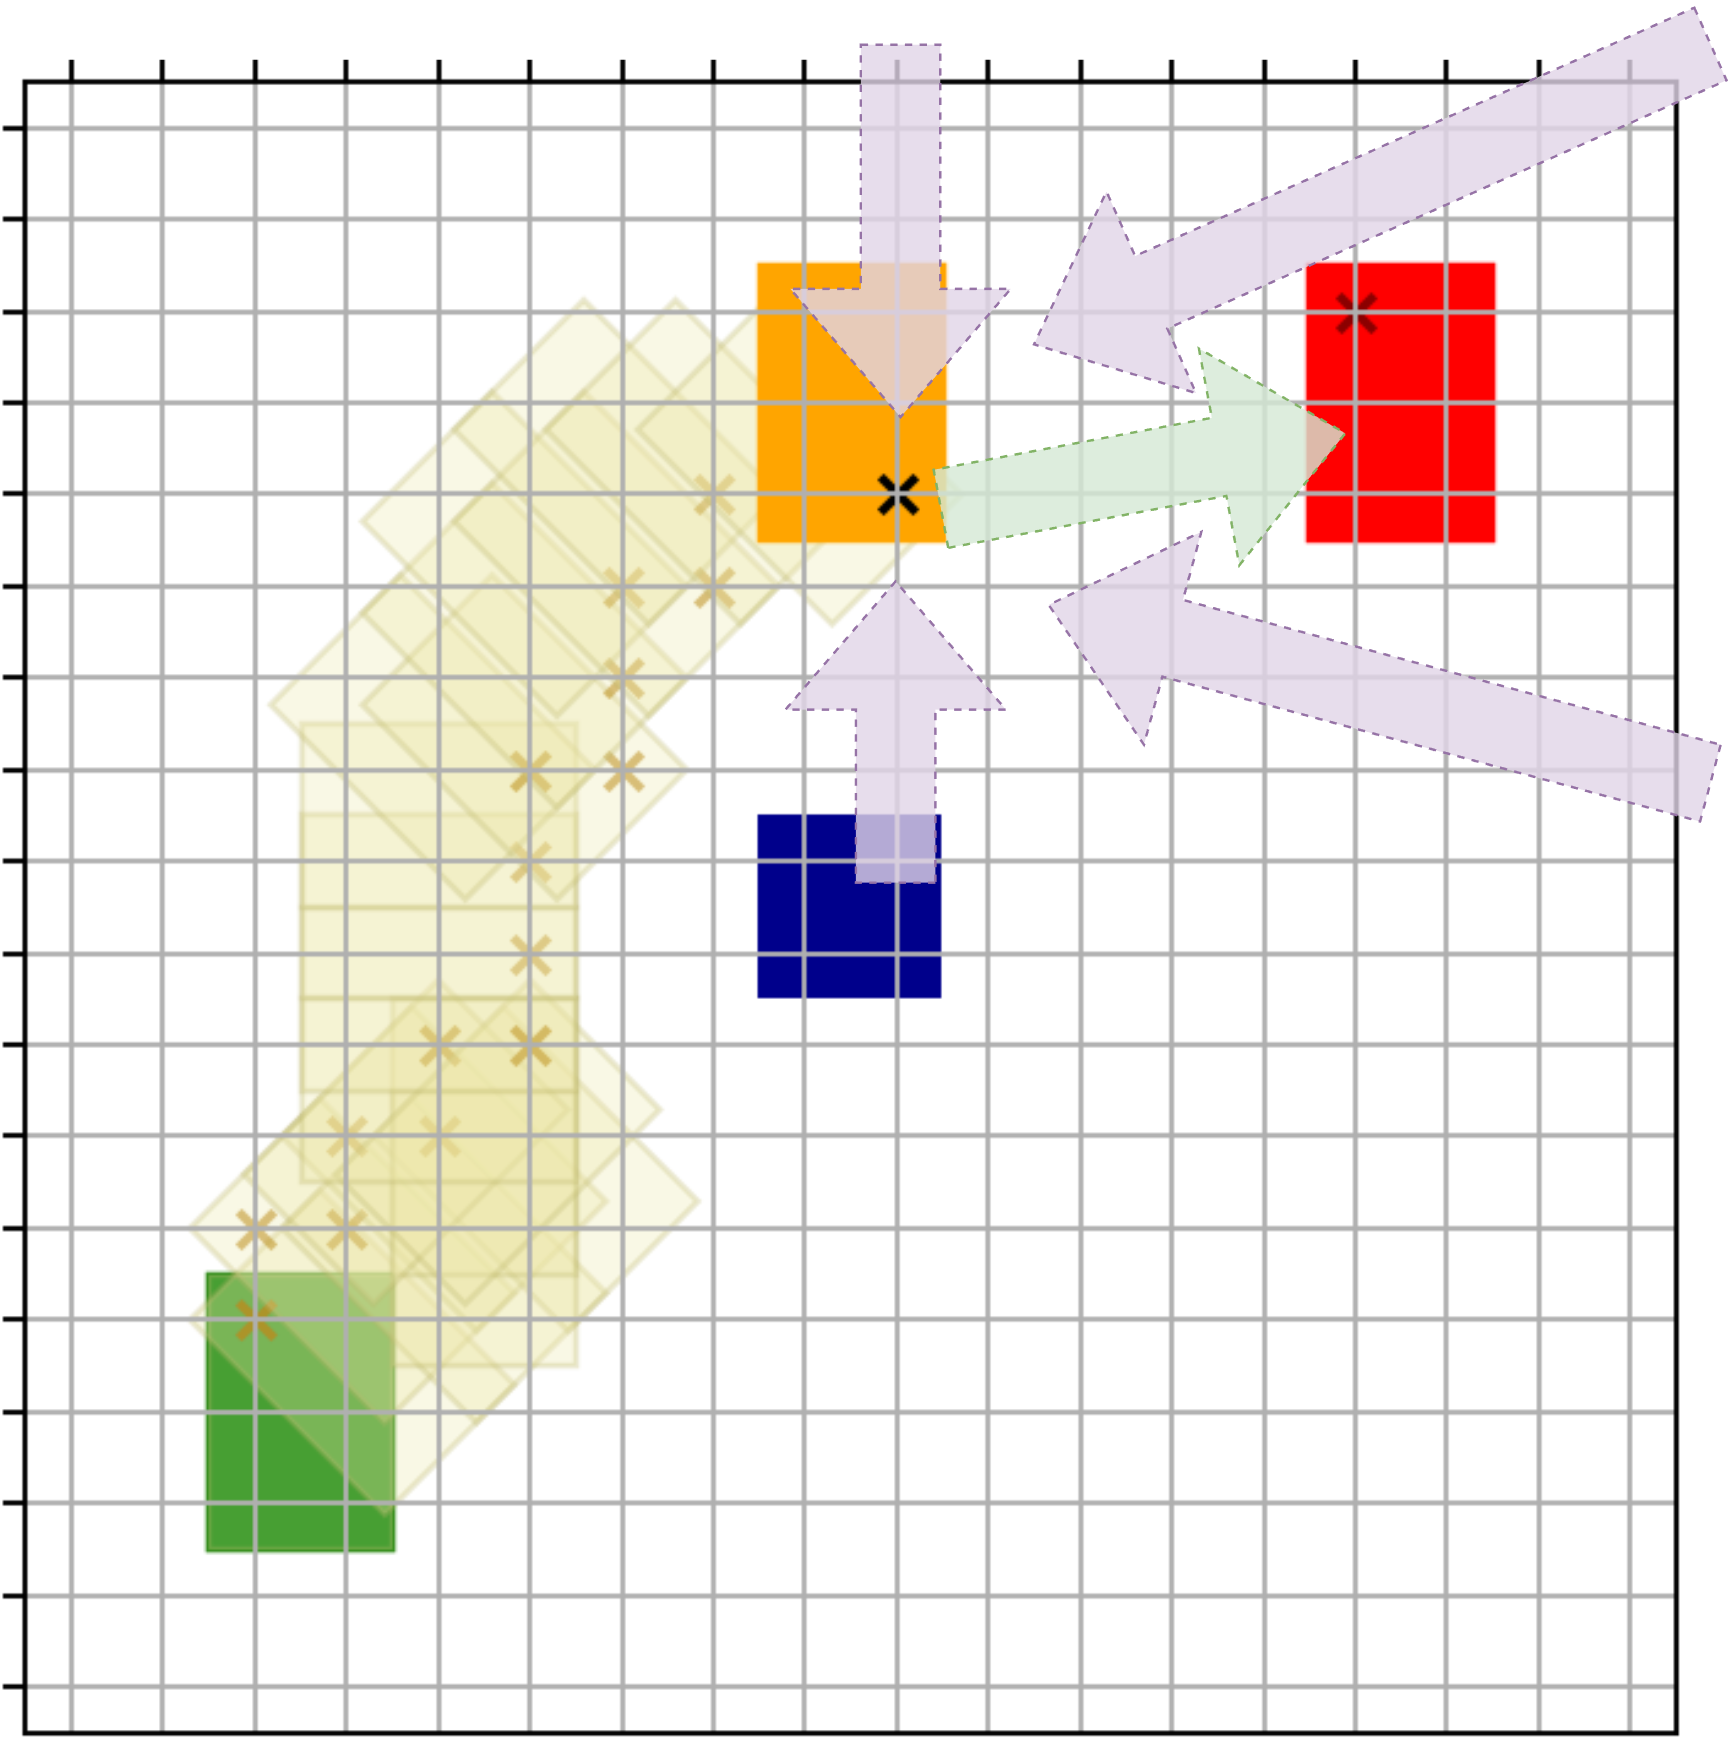
\includegraphics{bilder/attr-repul-oscillating-arrow.png}}}
	\end{minipage}
	\hspace*{\fill}
	\begin{minipage}{0.46\textwidth}%
		\footnotesize
		\centerline{\resizebox{0.6\linewidth}{!}{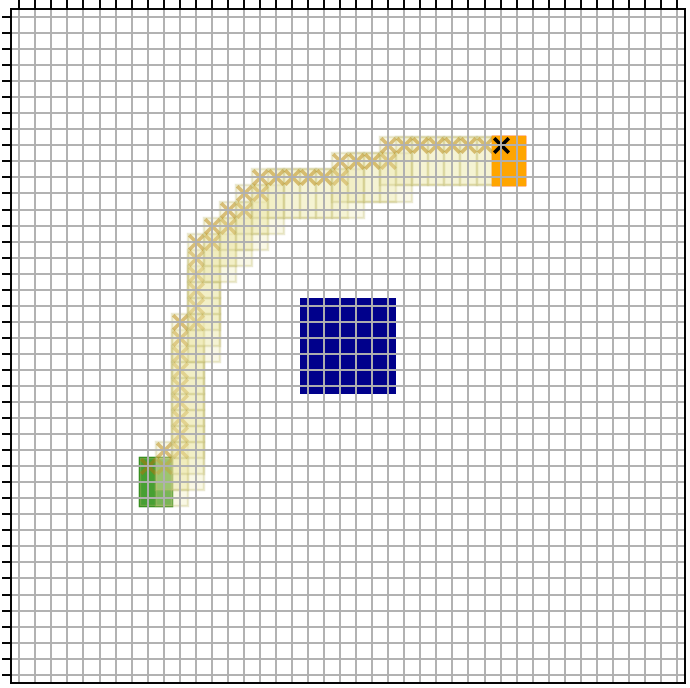
\includegraphics{bilder/attr-repul-oscillating-scaled.png}}}
	\end{minipage}
	\hspace*{\fill}
	%	\vspace{-1cm}
	\label{fig:oscillation}
	\caption{Bei Engstellen heben sich die abstoßenden Kräfte zwischen Hindernissen auf (links), bei hinreichend Abstand nicht (rechts).}
\end{figure}


Im Gegensatz dazu verhindert die streng monotone Potenzialänderung des Wavefront Algorithmus die Konvergenz zu lokalen Minima, sofern sich das Ziel an einem für den Roboter physikalisch erreichbaren Punkt befindet.

	- Konvergiert nie zu lokalem Minima
	- Potenziale nur in physikalisch erreichbaren Regionen definiert

*** TODO: Abbildungen mit unterschiedlichen Wavefront Szenarien ***


\section{Überdeckungen des Robotermodells mit Hindernissen}

Beobachtung bei den getesteten Szenarien der Implementierung: 
- Schlechte Interpolation der rotierten Robotermaske für kleine Roboterdimensionen mit kleinen Rotationsschritten in einem kleinen Occupancy Grids
 *** TODO: Beispiel Interpolation für 1x3 bei 10° ***

In Literatur (Author Wavefront) deshalb empfohlen: mit kleinen Rotationsschritten die Roboterdimensionen und das Occupancy Grid zu skalieren
=> Erhöht die Auflösung der Robotermaske, verringert Artefakte der Interpolation

*** TODO Beispiel Skalierung ***